\documentclass[twoside,twocolumn]{article}
\everymath{\displaystyle}
\usepackage{graphicx}
\usepackage{float}
\usepackage{blindtext} % Package to generate dummy text throughout this template 

\usepackage[sc]{mathpazo} % Use the Palatino font
\usepackage[T1]{fontenc} % Use 8-bit encoding that has 256 glyphs
\linespread{1.05} % Line spacing - Palatino needs more space between lines
\usepackage{microtype} % Slightly tweak font spacing for aesthetics

\usepackage[english]{babel} % Language hyphenation and typographical rules

\usepackage[hmarginratio=1:1,top=32mm,columnsep=20pt]{geometry} % Document margins
\usepackage[hang, small,labelfont=bf,up,textfont=it,up]{caption} % Custom captions under/above floats in tables or figures
\usepackage{booktabs} % Horizontal rules in tables

\usepackage{lettrine} % The lettrine is the first enlarged letter at the beginning of the text

\usepackage{enumitem} % Customized lists
\setlist[itemize]{noitemsep} % Make itemize lists more compact

\usepackage{abstract} % Allows abstract customization
\renewcommand{\abstractnamefont}{\normalfont\bfseries} % Set the "Abstract" text to bold
\renewcommand{\abstracttextfont}{\normalfont\small\itshape} % Set the abstract itself to small italic text

\usepackage{titlesec} % Allows customization of titles
\renewcommand\thesection{\Roman{section}} % Roman numerals for the sections
\renewcommand\thesubsection{\roman{subsection}} % roman numerals for subsections
\titleformat{\section}[block]{\large\scshape\centering}{\thesection.}{1em}{} % Change the look of the section titles
\titleformat{\subsection}[block]{\large}{\thesubsection.}{1em}{} % Change the look of the section titles

\usepackage{fancyhdr} % Headers and footers
\pagestyle{fancy} % All pages have headers and footers
\fancyhead{} % Blank out the default header
\fancyfoot{} % Blank out the default footer
\fancyhead[C]{Running title $\bullet$ May 2016 $\bullet$ Vol. XXI, No. 1} % Custom header text
\fancyfoot[RO,LE]{\thepage} % Custom footer text

\usepackage{titling} % Customizing the title section

\usepackage{hyperref} % For hyperlinks in the PDF

%----------------------------------------------------------------------------------------
%	TITLE SECTION
%----------------------------------------------------------------------------------------

\setlength{\droptitle}{-4\baselineskip} % Move the title up

\pretitle{\begin{center}\Huge\bfseries} % Article title formatting
\posttitle{\end{center}} % Article title closing formatting
\title{Precise Calculation of Electrical Capacitance by means of Quadruple Integrals in  Method of Moments technique} % Article title
\author{%
\textsc{Saeed Sarkarati}\thanks{A thank you or further information} \\[1ex] % Your name
\normalsize Shahid Beheshti University \\ % Your institution
\normalsize \href{mailto:saeedsarkarati@gmail.com}{saeedsarkarati@gmail.com} % Your email address
%\and % Uncomment if 2 authors are required, duplicate these 4 lines if more
%\textsc{Jane Smith}\thanks{Corresponding author} \\[1ex] % Second author's name
%\normalsize University of Utah \\ % Second author's institution
%\normalsize \href{mailto:jane@smith.com}{jane@smith.com} % Second author's email address
}
\date{\today} % Leave empty to omit a date
\renewcommand{\maketitlehookd}{%
\begin{abstract}
\noindent In this paper capacitance of parallel plate air gapped rectangular capacitor and unit cube have been calculated. Because of its generallity and simplicity MOM Technique is utilized. Due to precision increment, applying quadrauple integrals instead of double integrals has been suggested. A neat form for anlytical solution of integrals needed for MOM technique is presented. The results show very small error for capacitance calculation even with rough boundary tesselation. Described formulae and codes can easily be used for similar purposes.
\end{abstract}
}

%----------------------------------------------------------------------------------------

\begin{document}

% Print the title
\maketitle

%----------------------------------------------------------------------------------------
%	ARTICLE CONTENTS
%----------------------------------------------------------------------------------------

\section{Introduction}

\lettrine[nindent=0em,lines=3]{F} rom early  water-filled Leyden jar upto modern supercapacitors, precise calculation of capacitance is a challenging problem for scientists and researchers.

Electric capacitance of capacitors has been calculated by a variety of methods such as finite difference and finite element methods, monte carlo technique and method of moments. Except stochasic methods, the other ones make an equation matrix which must be solved to get the capacitance of desired geometry. Size of this matrix is a critical parameter resulting time needed for capacitance calculation.

If we concentrate on air gapped capacitors boundary element methods become best choice for calculation. In the lack of dielectic boundaries only air-metal boundaries must be considered. In method of moments (MOM) the elements are placed on boundary surfaces. And in special case of parallel plate air-gapped capacitor only two conducting plate surface are involved in generating matrix elements. So the matrix size is very small compard with matrix size in finite difference and finite element methods. Although these two techniques conclude sparse matrices, huge amount of their matrix sizes can not be compensated by using improved fast sparse matrix manipulation techniques. 

To do calculations in MOM it is needed firstly to make coupling matrix which consists of mutual and self coupling coeffitients between boundary segments or tiles. And then matrix equation must be solved. Various geometries for boundary segments have been suggested by authors. triangular tiles, square tiles, rectangular tiles and arbitrary shped tiles have been considered as boundary segments in MOM by researchers and scientists. 

To obtain coupling matrix coefficients, it is needed to integrate over segment plates. These integral calculations can be done numerically or analytically. Numerical integration can genarally be used for every segment. It can be done by stochastic or direct methods; and there are many optimised packages and libraries for doing it; But speed of calculation is obviously low against % ss 
using exact formulae obtaind from analytical calculations. In the other words we usually expect to spend cpu time for solving matrix equation, but numerical integration makes generating matrix time more larger %ss
. Although some authors have suggested mixed methods to obtain simplicity and speed together.

In this paper we have used an integral tranformation % nima
to solve quadruple integrals which give us exact formulae for coupling matrix coeffitients with no approximation. These analytical Terms %ss
have been used to generate coupling matrix. Matrix equation have been solved and electric capacitance has been calculated for parallel plate air gapped capacitor and the results have been compares with approximated integral calculation methods. Charge distribution over capacitor plates also has beeb investigated.

An undersandable path to solving quadrapule integrals and very neat form for analytical calculation are presented here to help researchers to calculate their own desired geometries.

A python code is written for doing the calculation and it is now available in our website and can be freely used by others. NUMPY and SCIPY libraries have been used to do numerical calculation easily and relatively %ss
 fast.
\section{Method of Moments for Capacitance Calculation}

Basic ideas for MOM technique firstly suggested by great physisist James Clarke Maxwell, who wanted to calculate electric capacity of a metall square. It is worth to have a look at his work which can be found here https://archive.org/details/

electricalresear00caveuoft/page/426.


He divided the square into 36 equal squares and assumed uniform charge density for each one, Then he assumed electric potential at the middle of each square segment equal to 1. To keep potential of all segments to one, electric charge of each segment must be different to others. There are 36 Values for 36 segments. but geometic symmetry shows us these 36 values can be grouped into 6 distinced values. 
\begin {figure}
\center
\begin{tabular}{ c c c c c c }
  A & B & C & C & B & A \\
  B & D & E & E & D & B \\
  C & E & F & F & E & C \\
  C & E & F & F & E & C \\
  B & D & E & E & D & B \\
  A & B & C & C & B & A \\
\end{tabular}
\caption{ss}
\end{figure}
He then calculuted electric charges of each segment and consequently electric capacitance.


Generally to calculate electric capacitance of a parallel plate capacitor, at first two constant voltage are proposed for two plate (usually 1V and -1V). Now each plate must be divided to segments. Electric potential of each segment must be equal to its plate. On the other hand potential of each segment can be calculated by means of electric charge of all segments and coupling coeffitients.
\begin{equation}
\label{eq1}
V_i = \sum_j P_{ij} Q_j
\end{equation}
This formula can be written in matrix form.
\begin{equation}
\label{eq2}
\mathbf V = \mathbf P \mathbf Q
\end{equation}
 Now it is needed to solve this matrix equation to calculate charge of each segment, And obviously capacitance can be obtained when electric potential and electric charge are known.
 
Coupling coeffitient between two segment depends on shape and location of two segments. It can be approximated roughly by potential formula of a unit point charge. 
\begin{equation}
\label{eq3}
P_{ij} = \frac{1}{4 \pi \epsilon_0\  d_{ij}}
\end{equation}
where $d_{ij}$ is the distance between centers of two segments.


In literature this approximation is used in a method called "surface charge simulation method", although this method can be categorized in varieties of MOM. Really for self coupling coeffitient this formula is not usefull. Self coupling is calculated by integrating over the area to find mean distance of all the points of area to its center.
\begin{equation}
\label{eq4}
P_{ii} = \frac 1 {S_i} \int \int \frac {dx\  dy}{4 \pi \epsilon_0 \sqrt{(x-x_{ci})^2 + (y-y_{ci})^2}}
\end{equation}
Where $(x_{ci}, y_{ci})$ is the center point of domain i and $S_i $ is the segment area.
To find out less approximated results in capactance calculation it is better to apply double integral formula, not only for self coupling, but also in mutual coupling. It leads us to double integral formulation.
\begin{equation}
\label{eq5}
P_{ij} = \frac 1 {S_i}\int \int \frac {dx\  dy}{4 \pi \epsilon_0 \sqrt{(x-x_{cj})^2 + (y-y_{cj})^2+ z_c^2}}
\end{equation}
Two domains are assumed to be parallel. Perpendicular plates will be investigated in succeeding sections of this paper. $z$ is  distance of two domains and is constant over integration. The integral must be calculated over domain i, and distance of each point to center of other domain is considered in this formula. These integrals can be calculated analythically and have been applied to find capacitance of parallel plate capacitors by nishiyama and nakamura.

Obviously this formula is not suitable where two domains are relatively close according to their dimensions. In this case we can not propose center of one domain as representative of all points. Really it is better to find all mutual distances between points of two segments. It can be done by using quadraple integral instead of double integral.
\begin{equation}
\label {eq6}
P_{ij} = \frac 1 {S_i S_j}\int \int \int \int \frac{dx_i dy_i dx_j dy_j}{4 \pi \epsilon_0 d_{ij}}
\end{equation} 
where $d _{ij}$ is 
\begin{equation}
\label {eq7}
d_{ij} = \sqrt{(x_i-x_j)^2 + (y_i-y_j)^2 + z_c^2}
\end{equation} 

\section{Quadruple Integration for Parallel Rectangular Segments}
To obtain coupling coeffitient described in Eq(6) one can use numerical integration method or solve it analytically. Although there are many improvements in numerical techniques, but analytical solutions still tke less process time. Firstly it is done by Eibert and Hansen for triangular domains. Analytical solution for rectangular domains presented by Lopez-Pena and Mosig, with a small mistake in driven formula. Recently this integral has been performed by Maccarrone and Paffuti, and its result has been used to find capacitance and forces for two square electrodes.

To perform integral in Eq(6) we can use this transformation.
\begin{equation}\label {eq8}
\frac 1 d_{ij} = \frac{2}{\sqrt{\pi}}\int_0^{\infty} e^{-u^2 d_{ij}^2 }du
\end{equation}
And Eq(6) can be rewritten in this form.
\begin{equation}
\label {eq9}
P_{ij} = \frac 2 {\sqrt{\pi} S_i S_j}\int_0^{\infty}\int \int \int \int \frac{e^{-u^2 d_{ij}^2 } dx_i dy_i dx_j dy_j}{4 \pi \epsilon_0 } du
\end{equation}
For simplicity we omit constants from formula.

\begin{equation}
\label {eq10}
I = \int_0^{\infty}\int \int \int \int e^{-u^2 d_{ij}^2} dx_i dy_i dx_j dy_j du
\end{equation}
There is no way to find primitive function of $e^{-u^2 d_{ij}^2}$ over these five integrals, but we can find primitive function over four inner integrals. If we assume J as the primitive function of quadraple integral.
\begin{equation}
\label {eq11}
J = \int \int \int \int e^{-u^2 d_{ij}^2 } dx_i dy_i dx_j dy_j  
\end{equation}
Then J can be calculated analytically.
\begin{eqnarray}\label {eq12}
\begin{array}{lll}

J = \frac{e^{-u^2(x^2+y^2+z^2)}}{4u^4}+\frac{\sqrt{\pi}e^{-u^2(y^2 + z^2)}x\; \mathrm{erf}(u x)}{4u^3}\\ \\
+\frac{\sqrt{\pi}e^{-u^2(x^2 + z^2)}y\; \mathrm {erf}(u y)}{4u^3}+\frac{\pi e^{-u^2 z^2}x\;y\; \mathrm{erf}(u x)\; \mathrm{erf}(u y)}{4u^2}
\end{array}
\end{eqnarray}
Where $x = x_i - x_j$ , $y = y_i - y_j$ and $z = z_c$\ . 
Now these integrals must be calculated seperately.
\begin{equation}\label {eq13}
\begin{array}{lll}

I_1& = &\big[\int_0^{\infty}\frac{e^{-u^2(x^2+y^2+z^2)}}{4u^4}\big]_{D_0}^{D_1}\\
I_2& = &\big[\int_0^{\infty}\frac{\sqrt{\pi}e^{-u^2(y^2 + z^2)}x\; \mathrm{erf}(u x)}{4u^3}\big]_{D_0}^{D_1}\\ 
I_3& = &\big[\int_0^{\infty}\frac{\sqrt{\pi}e^{-u^2(x^2 + z^2)}y\; \mathrm {erf}(u y)}{4u^3}\big]_{D_0}^{D_1}\\
I_4& = &\big[\int_0^{\infty}\frac{\pi e^{-u^2 z^2}x\;y\; \mathrm{erf}(u x)\; \mathrm{erf}(u y)}{4u^2}\big]_{D_0}^{D_1}
\end{array}
\end{equation}
We want to do calculation over rectangular segments. So limits of integration are over two rectangles.
\begin{eqnarray}\label {eq14}
D_0:\;\;x_i=a_0, y_i = b_0,\ x_j = c_0,y_j = d_0\nonumber\\
D_1:\;\;x_i=a_1, y_i = b_1, \ x_j = c_1,y_j = d_1
\end{eqnarray}
Finally the answer can be calcuted.
\begin{equation}\label {eq15}
\begin{array}{lll}

I_1 = \sum_{i,j,k,l=0}^1 A_{i,j,k,l}\frac {\sqrt{\pi} } {6} (x^2+y^2+z^2)^{\frac 3 2}\\
I_2 = \sum_{i,j,k,l=0}^1 -A_{i,j,k,l}\frac {\sqrt{\pi} } {4}\;x\ \times \\
\left((y^2 + z^2) \;\mathrm{sinh^{-1}}(\frac{x}{\sqrt{y^2 + z^2}}) +x \sqrt{x^2 + y^2 + z^2}\right)\\ 
I_3 = \sum_{i,j,k,l=0}^1 -A_{i,j,k,l}\frac {\sqrt{\pi} } {4}\;y\ \times \\
\left((x^2 + z^2)\;\mathrm{sinh^{-1}}(\frac{y}{\sqrt{x^2 + z^2}}) +y \sqrt{x^2 + y^2 + z^2}\right) \\ 
I_4 = \sum_{i,j,k,l=0}^1 A_{i,j,k,l}\frac {\sqrt{\pi} } {2}\;x\;y \left(x\;\mathrm{sinh^{-1}}(\frac{y}{\sqrt{x^2 + z^2}})+ \right.\\
\left. y\;\mathrm{sinh^{-1}}(\frac{x}{\sqrt{y^2 + z^2}}) -z\;\mathrm{tan^{-1}}(\frac{x\;y}{z\;\sqrt{x^2+y^2 + z^2}}) \right)\\ 

\end{array}
\end{equation}
In above expressions $x = a_i - c_j$ , $y = b_k - d_l\ $ and $z = z_c$. The amount of $A_{i,j,k,l}$ deponds on sum of i to l. If this summation is an odd number $A_{i,j,k,l}$ becomes -1, otherwise its value equals to 1.
\begin{equation}\label{eq16}
A_{i,j,k,l} = \Big\{^{\;\;1\quad  \mathrm{if}\; i + j + k + l\; \mathrm{is \;even}}_{-1\quad  \mathrm{if}\; i + j + k + l\; \mathrm{is \;odd}}
\end{equation}
Now it is needed to find sum of $I_1$ to $I_4$.
\begin{equation}\label {eq:17}
\begin{array}{ll}
I&=I_1+I_2+I_3+I_4 = \sum_{i,j,k,l=0}^1 A_{i,j,k,l}\\
&  \bigg[ \frac {\sqrt{\pi} } {12} \left((-x^2-y^2+2\;z^2)\sqrt{x^2 + y^2 + z^2} \right) \\

& \ +  \frac {\sqrt{\pi} } {4} \bigg( y(x^2 - z^2)\;\mathrm{sinh^{-1}}(\frac{y}{\sqrt{x^2 + z^2}}) \bigg)\\
&\ +   \frac {\sqrt{\pi} } {4}\left( x(y^2-z^2)\;\mathrm{sinh^{-1}}(\frac{x}{\sqrt{y^2 + z^2}})  \right)\\ 
&\ -  \frac {\sqrt{\pi} } {2}x \;y\;z\;\mathrm{tan^{-1}}(\frac{x\;y}{z\;\sqrt{x^2+y^2 + z^2}})\bigg]

\end{array}
\end{equation}
As we know $"\mathrm{sinh^{-1}}(x) = \mathrm{ln}(x+\sqrt{x^2 + 1})"$,
the above formula can be rewitten in this form.
\begin{equation}\label {eq:18}
\begin{array}{ll}
I&=\sum_{i,j,k,l=0}^1 A_{i,j,k,l}\left[\frac {\sqrt{\pi} } {12} \left((-x^2-y^2+2\;z^2)\sqrt{x^2 + y^2 + z^2} \right)\right.  \\

& + \frac {\sqrt{\pi} } {4} \bigg( y(x^2 - z^2)\;\mathrm{ln}(\frac{y+\sqrt{ {x^2 + y^2 + z^2}}}{\sqrt{x^2 + z^2}}\;)\\
&\ \ \ \ \ \ \ \ \ +x(y^2-z^2)\; \mathrm{ln}(\frac{x+\sqrt{ {x^2 + y^2 + z^2}}}{\sqrt{y^2 + z^2}}\;)  \bigg)\\ 
&- \left. \frac {\sqrt{\pi} } {2}x \;y\;z\;\mathrm{tan^{-1}}(\frac{x\;y}{z\;\sqrt{x^2+y^2 + z^2}} ) \right]

\end{array}
\end{equation}
In this paper we prefer to use hyperbolic form of formula, wich introduced in eq(17).
In the case that two segments are coplanar, mutual coupling obtains by taking limit of eq(17) when $z$ goes to zero.
\begin{equation}\label {eq:19}
\begin{array}{l}
I_{coplanar}=\sum_{i,j,k,l=0}^1 A_{i,j,k,l}\left[\frac {\sqrt{\pi} } {12} \left((-x^2-y^2)\sqrt{x^2 + y^2} \right) \right. \\

 + \left. \frac {\sqrt{\pi} } {4} \left( y(x^2 )\;\mathrm{sinh^{-1}}(\frac{y}{x })+x(y^2)\;\mathrm{sinh^{-1}}(\frac{x}{y})  \right) \right]
\end{array}
\end{equation}
Implementaion of this formula needs special attention to the cases which any denominator of fractions becomes zero. Easily each term, involving such fractions goes to zero and can be omitted in calcalulation.


And finally self coupling of a rectangular segment takes this form.

\begin{equation}\label {eq:20}
\begin{array}{l}
I_{SC} = \frac {\sqrt{\pi} } {3} (x^3+y^3)
+ \frac {\sqrt{\pi} } {3} \left((-x^2-y^2) \sqrt{x^2 + y^2} \right)\nonumber \\ +\sqrt{\pi} \left( y(x^2 )\;\mathrm{sinh^{-1}}(\frac{y}{x})+x(y^2)\;\mathrm{sinh^{-1}}(\frac{x}{y})  \right)
\end{array}
\end{equation}

Now x and y are length and widh of rectangular region.
\section{Quadruple Integration for Perpendicular Rectangular Segments}
Coupling coeficient for perpendicular segments can be obtained by this formula.

\begin{equation}
\label {eq21}
P_{ij} = \frac 1 {S_i S_j}\int \int \int \int \frac{dx_i dy_i dx_j dz_j}{4 \pi \epsilon_0 d_{ij}}
\end{equation} 
where $d _{ij}$ is 
\begin{equation}
\label {eq22}
d_{ij} = \sqrt{(x_i-x_j)^2 + (y_i-y_c)^2 + (z_c - z_j)^2}
\end{equation} 
Where $z_c$ and $y_c$ are constants in integration. With similar transformation utilized for parallel plates, primitive function of quadraple integral can be obtained.
\begin{eqnarray}
\label {eq23}
\begin{array}{lll}

J = \frac{\pi\sqrt{\pi}\;x\; \mathrm {erf}(u x)\; \mathrm {erf}(u y)\; \mathrm {erf}(u z)}{8u^3}\\
+\; \frac{\pi e^{-u^2 x^2} \mathrm{erf}(u y)\; \mathrm{erf}(u z)}{8u^4}
\end{array}
\end{eqnarray}
%------------
Where $x = x_i - x_j$ , $y = y - y_j$ and $z = x_i - x_j$\ .
And finally coupling coefficient of two perpendicular plate is obtained.
\begin{equation}\label {eq:24}
\begin{array}{ll}
I& = \sum_{i,j,k,l=0}^1 A_{i,j,k,l}\\
&  \bigg[ -\frac {\sqrt{\pi} } {6} \left((y\; z)\sqrt{x^2 + y^2 + z^2} \right) \\

& +\  \frac {\sqrt{\pi} } {12} \bigg( z(3x^2 - z^2)\;\mathrm{sinh^{-1}}(\frac{y}{\sqrt{x^2 + z^2}}) \bigg)\\
& +\  \frac {\sqrt{\pi} } {12} \bigg( y(3x^2 - y^2)\;\mathrm{sinh^{-1}}(\frac{z}{\sqrt{x^2 + y^2}}) \bigg)\\
& +\  \frac {\sqrt{\pi} } {2} \bigg( x\; y\; z\;\mathrm{sinh^{-1}}(\frac{x}{\sqrt{y^2 + z^2}}) \bigg)\\
&-  \frac {\sqrt{\pi} } {4}\;x \;z^2\;\mathrm{tan^{-1}}(\frac{x\;y}{z\;\sqrt{x^2+y^2 + z^2}})\\

&-  \frac {\sqrt{\pi} } {4}\;x \;y^2\;\mathrm{tan^{-1}}(\frac{x\;z}{y\;\sqrt{x^2+y^2 + z^2}})\\
&-  \frac {\sqrt{\pi} } {12}\;x^3\;\mathrm{tan^{-1}}(\frac{y\;z}{x\;\sqrt{x^2+y^2 + z^2}})\bigg]

% @@@@@@@@@@@

\end{array}
\end{equation}
Now in above expressions $x = a_i - c_j$ , $y = b_k - y_c\ $ and $z = z_c - d_l$.

\section{Results}
For test correctness of analytical results firstly they have been compared with results of numerical integration in some domains. A complete agreement and zero error occured. Although because of singularities numerical integration can not be done easily for every domain of integration. For test capability of results two classical problems solved with these formulae: Capacitance of parallel plate air gapped capacitor and Capacitance of unit cube.


\begin {figure}[h]
	\center
	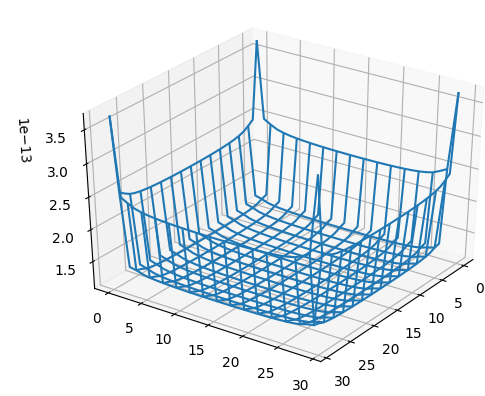
\includegraphics[width=\linewidth]	{wired.png}
	\caption{Charge distribution on one plate of parallel plate plate air gapped capacitor}
\end{figure}
As mentioned above in MOM a set of equation is solved to obtain charge amount of every tile. So charge density distribution is obtained directly in this method. As an example this method applied to an air gapped parallel plate capacitor with  $1m \times 1m $ plate dimensions and a plate seperation of 10 cm. In fig. 2 charge distribution has been showed. Calculation of chare density in some research areas such as high voltage engineering is a bottleneck of designing apparatus.


Capacitance of parallel plate air gapped capacitor has been calculated in three methods. In the first one, point charge approximation is used for mutual coupling and double integration for self coupling. In the second mehod both of self and mutual couplings are calculated by means of double integration. The third method uses quadraple integration for calculating coupling coeffitients. 
\begin {figure}[h]
	\center
	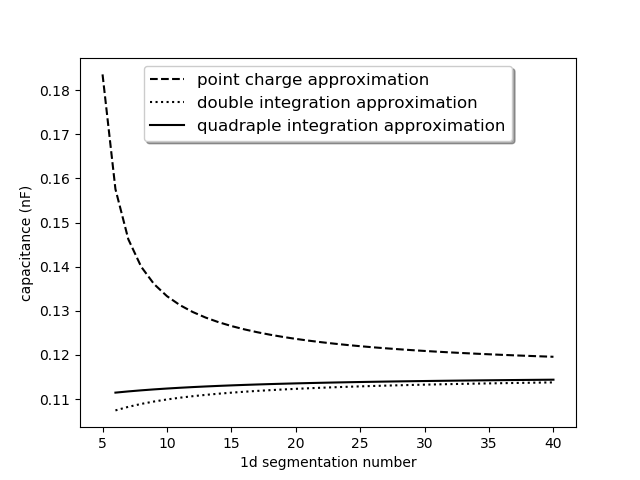
\includegraphics[width=\linewidth]	{saeedvshitoshiandzho.png}
	\caption{Capacitane of quadraple integration vs two other methods}
\end{figure}

In fig.3 results of capacitance extraction are shown for these three methods versus number of segmentation of square plate in each dimension (n). Total number of tiles is 2 * n * n. Because of far answers of point charge method in small number of segmentation, the first five results are omitted. It can be seen that point charge approximation is out of accuracy and two others are more compatible. 
\begin {figure}[h]
	\center
	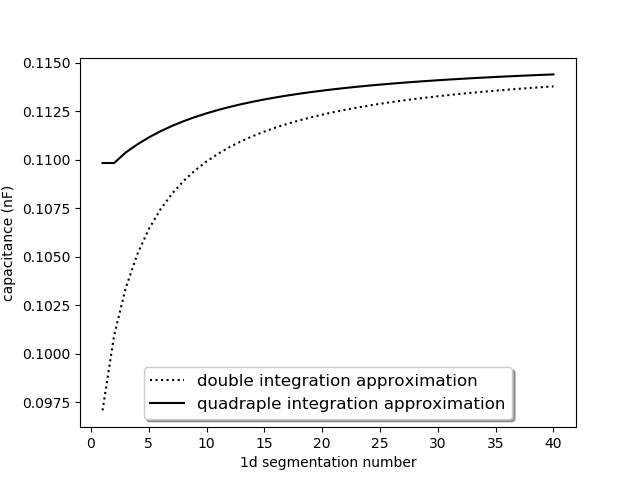
\includegraphics[width=\linewidth]	{saeedvshitoshi.png}
	\caption{comparsion between results extracted from double and quadraple integrations}
\end{figure}

In fig.4 double and quadraple integration methods are compared. Clearly quadraple integration results more accurate advantages. Even in rough segmentations a meaningful answer has been achieved from quadraple integration.

\begin {figure}[h]
	\center
	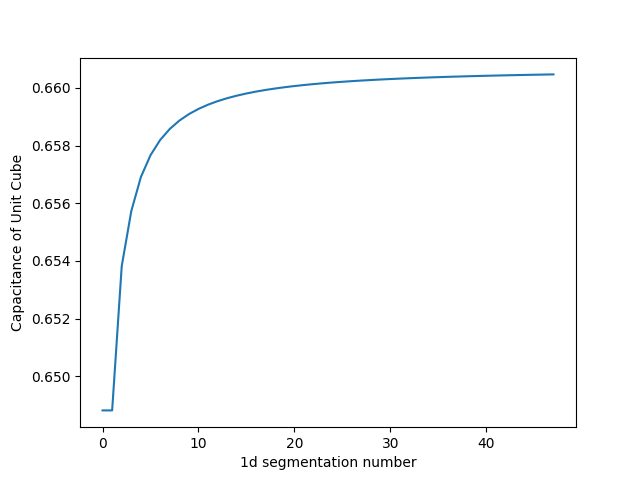
\includegraphics[width=\linewidth]	{unitcube.png}
	\caption{Capacitance if unit cube in units of $4\pi \epsilon_0$}
\end{figure}
The last investigated problem is Capacitance of unit cube. It is an old problem in electrostatics which can not be solved exactly. Many aouthors have tried different methods to solve this problem since 1950. We tried our analytical results for extracting matrix elements needed for method of moments. this results in 73.385 pF for 48 segment in each dimension i.e. 48 * 48 * 6 tiles totally. Most of the authors report this amount in units of $4\pi \epsilon_0$. It means that this amount must be multiplied by $9 \times 10^9$ and results in 0.66047, which is very close to best claimed amount i.e. 0.660678. The amount of capacitance have been drawn versus 1d segmentation in fig.5.

This chart shows not only good results in fine segmentation but also acceptable results in coarse segmentation. even if we consider each face of the cube as one segment, it yields less than 2 pecent error.
\end{document}
